\documentclass[../../preview.tex]{subfiles}
\begin{document} 
\begin{figure}
\centering
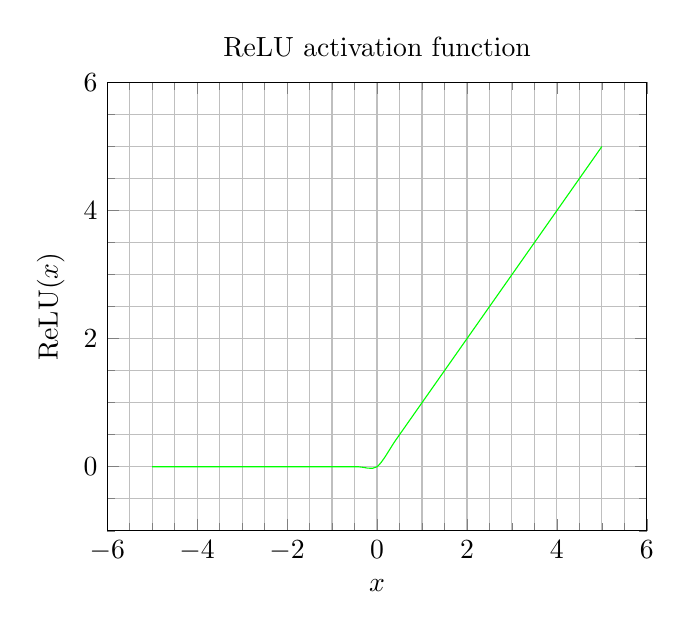
\begin{tikzpicture}
    \begin{axis}[
      title=ReLU activation function,
      xlabel={$x$},
      xmin=-6,
      xmax=6,
      minor x tick num=3,
      ylabel={$\textnormal{ReLU}(x)$},
      ymin=-1,
      ymax=6,
      minor y tick num=3,
      grid=both,
      ]
      \addplot[green,smooth] {max(0, x))};
    \end{axis}
  \end{tikzpicture}
\end{figure}
\end{document}
